\subsection{Experimentación preliminar}

\subsubsection{Idea}

Para concluir este trabajo, tomamos el algoritmo de backtracking, el algoritmo goloso, el de búsqueda local 1 y GRASP 1 y mediremos las diferencias de performance y de tiempos en cada uno para intentar sacar conclusiones.

Comenzaremos con un pequeño experimento variando $n$. Tomaremos grafos completos con $k = 5$, pesos aleatorios en las aristas y variando la cantidad de nodos desde $1$ a $19$ y mediremos cuales son los k-PMP encontrados por cada algoritmo.

\subsubsection{Experimentación}

Los resultados arrojados por la experimentación pueden verse en el siguiente gráfico:

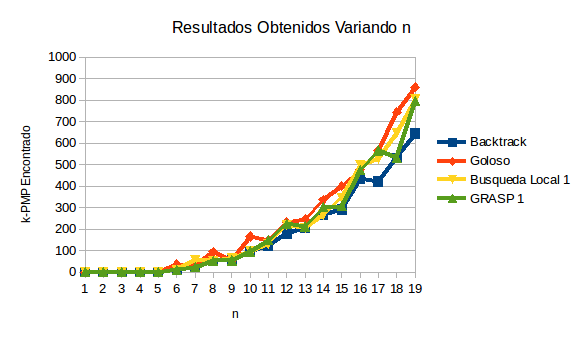
\includegraphics[scale=0.7]{Con/performance1.png}

Lo primero que podemos observar es que para casos triviales con $n <= k$ todos son capaces de encontrar la respuesta óptima.

Lo segundo que podemos observar, es que salvo un caso, el algoritmo goloso siempre pareciera ser el que encuentra las peores soluciones, llegando a obtener una respuesta un $33 \%$ alejada de la óptima en el caso de $19$ nodos. (k-PMP encontrado por el backtrack: 644, k-PMP encontrado por la heurística golosa: 860).

Las respuestas obtenidas por la búsqueda local y el GRASP, resultan en general, en mucho mejores k-PMPs, desviándose hasta un $10\%$ de la respuesta por backtracking.

Además de estos 19 casos, podemos ver que el algoritmo goloso encuentra $6$ soluciones exactas (las 5 triviales y una para $n = 9$), la búsqueda local encuentra $10$ respuestas exactas y el GRASP encuentra $11$ respuestas exactas. Si bien este el set de datos no es muy significativo, ya es posible ver las ventajas que representan las dos ultimas heurísticas frente a la primera.

Además, para estos 19 casos, medimos los tiempos que tardan en obtener una respuesta:

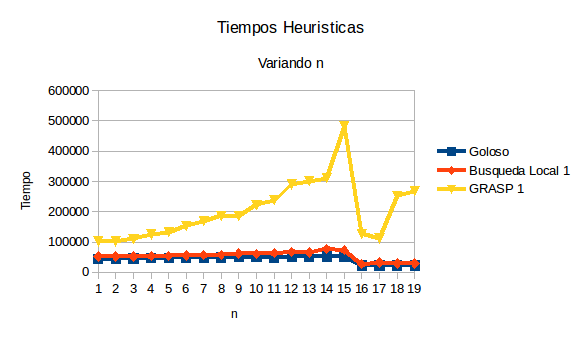
\includegraphics[scale=0.7]{Con/tiempos1Back.png}

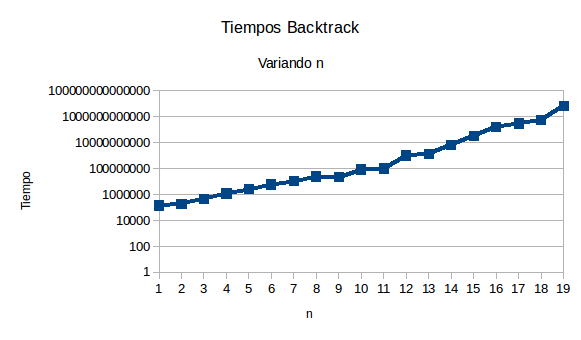
\includegraphics[scale=0.7]{Con/tiempos1Otros.png}

Como era de esperar, mientras que las heurísticas escalan de manera mas o menos polinomial, el backtracking escala de manera exponencial ascendiendo un orden de magnitud cada vez que asciende en uno el valor de $n$, hasta el punto que pasados los $19$ nodos, los tiempos empiezan a ser inviables.

\subsubsection{Conclusión}


En casos como el GRASP, por lo visto en las comparaciones, es el que mas se acerca en soluciones al backtracking aunque en algunas soluciones se nota como influye la busqueda local ya que se acerca mas a la busqueda local para grafos no muy densos, mientras crece mas el grafo es mas notorio, a diferencia del algoritmo goloso que se aleja mas de la solucion optima y resulta no ser una buena alternativa.\\
Podemos concluir que dependiendo de las heuristicas en algunos casos podriamos combinarlas para encontrar buenas soluciones al problema, en otros casos acercarnos a la optima con una gran diferencia de tiempo comparando con el algoritmo exacto. \\ Por la diferencia de tiempos podriamos seguir aplicando heuristicas para obtener mejores soluciones en el caso que sea factible, de esta manera acercarnos a la mejor solucion lo mas posible siempre y cuando los tiempos no sean parecidos al backtracking, en tal caso no tendria sentido porque por el mismo tiempo tendriamos la solucion optima.


\subsection{Experimentación sobre grafos Fáciles}

\subsubsection{Idea}

En esta sección buscaremos determinar cuanto mejor es el GRASP sobre la familia de grafos para la que fue entrenada (grafos completos, con aristas tomadas al azar entre $1$ y $100$) y que consideramos que será sobre la cual tenga mejor desempeño. De esta manera intentaremos mostrar las ventajas que representa frente a los otros algoritmos. Para eso correremos el Backtrack sobre $100$ grafos de $18$ nodos completos, con pesos en las aristas aleatorios entre 1 y 100 y $k = 4$ y veremos en cuantos casos cada algoritmo encuentra la respuesta exacta, e intentaremos sacar conclusiones sobre los datos obtenidos.

\subsubsection{Experimentación}

De las respuestas arrojadas por el testing podemos sacar las siguientes conclusiones. El algoritmo Goloso logró encontrar una respuesta exacta, al comparar los resultados del mismo con las de backtracking. El algoritmo de búsqueda local y el GRASP, lograron encontrar 6 respuestas correctas cada uno.

Por otra parte, para cada respuesta obtenida por una heurística, sacamos el porcentaje de que tan alejada se encontraba de la respuesta exacta, y luego promediamos los valores para cada una de las heurísticas. Lo que obtuvimos fue que, en promedio, la búsqueda local se aleja un $25 \%$ de la respuesta exacta con un desvío estándar igual a $9$. La búsqueda local se aleja un $12 \%$ de la respuesta exacta con un desvío estándar igual a $9$ y el GRASP se aleja un $11 \%$ de la respuesta exacta con un desvío estándar igual a $8$.

\subsubsection{Conclusión}

Lo que podemos concluir de estos resultados es que el GRASP no solo obtiene mejores resultados sino que la dispersión de los mismos también es menor en comparación con los demás algoritmos. 

\subsection{Experimentación sobre grafos difíciles}

\subsubsection{Idea}

Para poner realmente a prueba las tres heurísticas diseñamos una nueva familia de grafos que consideramos difícil de resolver para nuestros algoritmos. Los grafos de esta familia se describen así: dada una cantidad de nodos $n$ y una cantidad de aristas igual a $n*(n-1)/2$, tomamos la mitad de las aristas con peso igual a $1$ y la otra mitad con peso igual a $100000$. Además k debe ser igual a $n/6$.

\subsubsection{Experimentación}

Fijamos $n=250$ y tomamos $100$ de estos grafos. Para ejemplificar lo obtenido, se incluyen las respuestas obtenidas en tres instancias del problema.

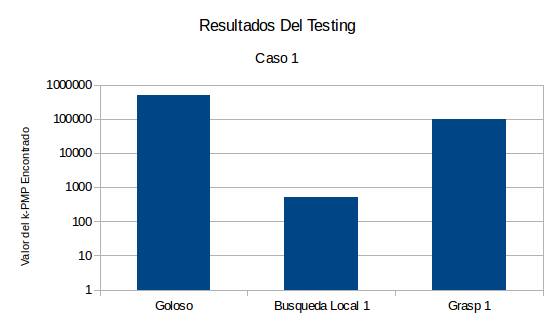
\includegraphics[scale=0.7]{Con/dificil1.png}

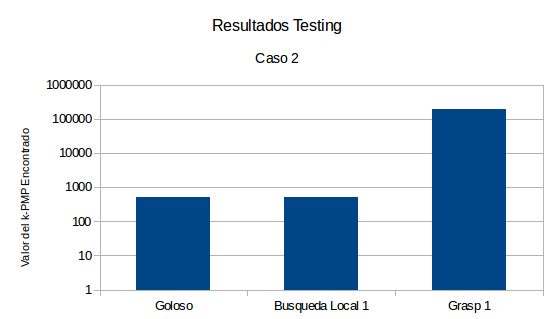
\includegraphics[scale=0.7]{Con/dificil2.png}

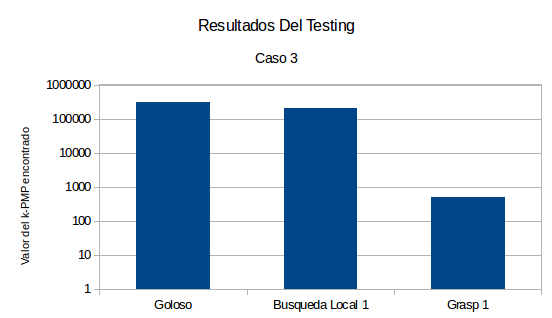
\includegraphics[scale=0.7]{Con/dificil3.png}

Notar que los gráficos están en escala logarítmica, lo que quiere decir, que en el caso uno por ejemplo, el algoritmo goloso (k-PMP encontrado: 500502) y el GRASP (k-PMP encontrado: 100501) obtuvieron respuestas aproximadamente un $100100 \%$ peor que la Búsqueda local (k-PMP encontrado: 501).

Llamaremos a una respuesta, "buena", si se encuentra entre $0$ y $1000$. Notar que una respuesta puede ser "buena", pero no necesariamente ser la respuesta exacta para el k-PMP. Para esta cantidad de vértices, ya es imposible encontrar una respuesta por backtracking.

Analizando los datos, vemos que el algoritmo goloso solo logró llegar a una respuesta buena, 4 veces, mientras que el tanto el GRASP, como la búsqueda local lograron obtener $51$ respuestas buenas en estos grafos (no necesariamente en el mismo grafo, como puede notares en las figuras)

\subsubsection{Conclusión}

Si bien un $50 \%$ de respuestas buenas puede ser una cantidad aceptable, una posible idea para mejorar aun mas los resultados, sería entrenar nuevamente al GRASP con este set de datos, y intentar conseguir un nuevo $\alpha$ y un nuevo $z$ de tal manera que se maximicen las posibilidades de encontrar la respuesta. Otro posible solución sería encontrar alguna propiedad especifica para esta familia de grafos que facilite su resolución con alguna otra heurística mas apropiada.

\section{Conclusiones Generales y Trabajo Futuro}

Concluimos que dado que el problema de $k-PMP$ resulta extremadamente difícil de resolver de manera exacta, es posible encontrar heurísticas que nos aproximen a una buena solución en un tiempo razonable, siempre teniendo en cuenta que pagamos tiempo con exactitud.

Vimos que la técnica de Metaheuristica GRASP es una combinación válida entre distintos esquemas de algoritmos y trata de combinarlas para explorar el espacio de soluciones de una manera eficiente. En nuestro caso particular vimos que la implementación de GRASP 1, lograba ser bastante efectivo dentro de la familia de grafos para las fue entrenado. Aunque como se vio en el apartado de "Experimentación sobre un grafo difícil" al ser utilizado para resolver casos patológicos, puede obtener respuestas equiparables con un algoritmo mas simple de búsqueda local.

Como trabajo futuro, podría intentar implementarse un backtracking que primero corra una buena metaheuristica de manera de comenzar con una buena solución inicial. De esa manera, las podas que podría aplicar el algoritmo, serían en teoría mucho mejores, lo que sin duda ayudaría a bajar los tiempos de ejecución.
